\documentclass[11pt]{article}

\usepackage[margin=1in]{geometry}
\usepackage{amsmath, amssymb}
\usepackage{graphicx}
\usepackage{booktabs}
\usepackage{microtype}
\usepackage{hyperref}
\usepackage{xcolor}
\usepackage{tikz}
\usepackage[most]{tcolorbox}
\usetikzlibrary{arrows.meta, positioning, decorations.pathreplacing,
                calc, shapes.geometric, patterns}

\graphicspath{{figures/}}

\hypersetup{colorlinks=true, linkcolor=blue!50!black,
            urlcolor=blue!50!black, citecolor=blue!50!black}

\newtcolorbox{numbersbox}[1][]{
  colback=blue!5, colframe=blue!50!black, fonttitle=\bfseries,
  title=#1, sharp corners, boxrule=0.6pt}

\newtcolorbox{primerbox}[1][]{
  colback=yellow!10, colframe=orange!70!black, fonttitle=\bfseries,
  title=#1, sharp corners, boxrule=0.6pt}

\title{Auditory Superstitious-Perception: results walkthrough}
\author{}
\date{}

\begin{document}
\maketitle
\tableofcontents
\bigskip

%==============================================================================
\section{The experiment}
%==============================================================================

26 college students completed two blocks of 149 trials each. On every
trial they heard a short noisy audio clip and reported whether it was the
``target'' or the ``distractor''. The underlying target and distractor
clips are essentially noise; chance performance is $0.50$.

The task revolves around listening for a target word (``wall'') in the context of a target sentence (``The picture hung on the wall'').
We cut out the final word (``wall'') and the stimuli are white noise audio clips with the
same length ($370 \text{ms}$), sampling rate ($8000 \text{Hz}$), and channel count ($1 \text{- Mono}$) as the extracted ``wall'' clip. 

There are target stimuli and distractor stimuli.
Target stimuli are more correlated (according to Pearson R) with the ``wall'' clip than the distractor stimuli are.
The question is whether, and under what circumstances, subjects can pick up on the correlation between
the target stimuli and the missing word, and correctly categorize white noise stimuli into target vs.\ distractor.

There were two block types. These are labelled \texttt{full\_sentence} and \texttt{imagined\_sentence}. 
In the \texttt{full\_sentence} block subjects hear the beginning of the target
sentence (``The picture hung on the'') followed by one of the white noise stimuli on each trial.
In the \texttt{imagined\_sentence} blocks subjects must imagine the beginning of
the sentence (e.g.\ ``The picture hung on the wall'') and then click a button to hear the white noise stimulus.


Subjects were recruited at Oberlin ($n = 16$) and UChicago ($n = 10$). Every comparison is reported three ways: each site
alone and pooled (``Unified'').

%==============================================================================
\section{Brief jargon primer}
%==============================================================================

Skip if you already know what a $p$-value, Cohen's $d$, and cosine
similarity are.

\subsection{Accuracy and chance}
Considering each subject's performance as a proportion of stimuli called correctly between 0 and 1 calculated via $\frac{\textbf{Correct Responses}}{\textbf{Total Stimuli Presented}}$. 
If subjects were guessing or at chance, then we would expect scores to cluster around $0.50$.

The intuition: imagine flipping a fair coin 150 times and calling each
flip. You will get close to 75 right but almost never exactly 75. By
chance alone you might land at 80/150 ($0.533$) or 70/150 ($0.467$).
That random spread around $0.50$ is what a single subject looks like
under the null. The question for each group is whether the cloud of
subject means sits noticeably to the right of $0.50$ \emph{more often
than that random spread would explain}.

Each subject completed $N = 149$ trials, with either 75 targets and 74 distractors or vice versa. 
Under a guessing model with no systematic knowledge (i.e., $d' = 0$), but allowing an arbitrary response bias $b = P(\text{``target''})$, 
the expected accuracy is

\[
E[\text{accuracy}] = \frac{K b + (N-K)(1-b)}{N},
\]

where $K$ is the number of targets. For $K = 75$ this simplifies to $(74 + b)/149$, and for $K = 74$ to $(75 - b)/149$. 
Because the class imbalance is only one trial, the expected accuracy remains extremely close to $0.5$ for any $b$ 
(maximum deviation $\approx 0.003$).

The variance of accuracy under this null is driven by trial-to-trial guessing variability. Since each trial is correct with probability 
approximately $0.5$, the standard deviation of a single subject's accuracy is

\[
\sqrt{\frac{0.5(1-0.5)}{149}} \approx 0.041.
\]

Thus, a single subject scoring $0.54$ falls well within the range expected by chance. However, for a group of $n = 16$ subjects, 
the standard error of the mean decreases by a factor of $\sqrt{n}$:

\[
\text{SE} = \frac{0.041}{\sqrt{16}} \approx 0.010.
\]

Consequently, a group mean of $0.526$ is substantially less likely to arise under the null than an individual deviation of similar magnitude.

We are interested to make a judgement about whether or not the subject responses are better explained by this null "guessing hypothesis" or by some other hypothesis, namely that subjects are able to do this task above chance.

Put graphically, does the cloud of points below fall above the mean in a reliable way that would be unlikely if subjects were just guessing? The red dashed line at $0.50$ is the null value; the blue points are individual subjects;
\begin{center}
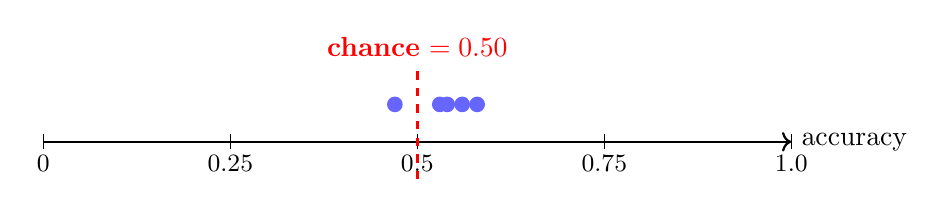
\begin{tikzpicture}[scale=0.95]
  \draw[thick,->] (0,0) -- (10,0) node[right]{accuracy};
  \foreach \x/\lab in {0/0, 2.5/0.25, 5/0.5, 7.5/0.75, 10/1.0}
    \draw (\x,-0.1) -- (\x,0.1) node[below=4pt]{\small \lab};
  \draw[red, very thick, dashed] (5,-0.5) -- (5,1.0)
        node[above, red]{\textbf{chance} $= 0.50$};
  \node[circle, fill=blue!60, inner sep=2pt] at (5.4,0.5) {};
  \node[circle, fill=blue!60, inner sep=2pt] at (5.6,0.5) {};
  \node[circle, fill=blue!60, inner sep=2pt] at (5.8,0.5) {};
  \node[circle, fill=blue!60, inner sep=2pt] at (5.3,0.5) {};
  \node[circle, fill=blue!60, inner sep=2pt] at (4.7,0.5) {};
\end{tikzpicture}
\end{center}

\subsection{The $p$-value}
Probability of a result at least as extreme as the observed one, under
the null hypothesis. Smaller $p$ = more surprising under the null. The
conventional cutoff is $p < 0.05$. 

The typical intuition and story you can tell yourself: Pretend the null is true (subjects are guessing). Now
imagine re-running the whole experiment a million times in that
imaginary world where the null is true. A two-tailed $p$-value is the proportion of those imaginary
experiments where the group mean is more than x percent away from the expected mean (either more the x percent below the mean or x percent above the mean).
A one-tailed $p$-value is the same, except you are asking \textbf{either} roportion of those imaginary
experiments where the group mean is x percent \textbf{greater} than the expected mean \textbf{or} the proportion where the group mean is x percent \textbf{less} than the expected mean, depending on the direction of your alternative hypothesis.

A $p$-value of $p = 0.05$ means \emph{1 in 20 imaginary null-world experiments would look this extreme by accident}.
A $p$-value of $p = 0.001$ means \emph{1 in 1000 imaginary null-world experiments would look this extreme by accident}.

The one-tailed $p$-value is always half the two-tailed $p$-value, because it only counts one of those tails. It is tempting to use one-tailed tests because it automatically cuts your $p$-value in half, but you should only do it if you have a strong theoretical reason to expect the effect to go in one direction and not the other. 
In this experiment, we took an exploratory data analysis approach and we did not have a sttrong enough hypothesis to justify a one-tailed test. As a result, all of the analyses we ran were two-tailed. This is the safest way to make sure that we took all precautions to avoid false positives, and it is the most conservative approach. 

A $p$-value is \emph{not} the probability that the null is true, and
it is \emph{not} the probability that the effect is real. It is a
statement about how often pure noise would mimic the observation.

When we run many tests (e.g.\ 6 cells in Section~A, 48 correlations in
Section~F) some will land below $0.05$ by accident. The more tests you run, the more likely you are to see a false-postive.
If you run enough tetsts, then you will expect to see one or more false-positive. 
If you roll a 20 sided die then you don't typically expect to roll a 4. But if you roll the die 1000 times then you expect to see \textit{some} 4s.
We correct for this using a conservative $p$-value correction known as Bonferroni correction. The Bonferroni 
correction divides our significance level $\alpha = 0.05$ by the number of tests; so if we run 6 tests then we take $\alpha = \frac{0.05}{6} = 0.0083$ as our new threshold for significance; if we run 48 tests then we take $\alpha = \frac{0.05}{48} \approx 0.001$ as our new threshold for significance. 

\subsection{Which $p$-test, and why}

A $p$-value always answers the same conceptual question (``how often would noise alone fake this?'') but \emph{how} it computes that depends on what kind of comparison you're making and what you're willing to assume about your data. The Results section uses a handful of different tests; here is what each one is doing and why we picked it.

A quick word on \emph{parametric} vs \emph{non-parametric} before we go through them. A parametric test (like Welch's $t$-test) assumes the data come from a particular shape of distribution --- usually a bell curve. If that assumption holds, you get a bit of extra statistical power. A non-parametric test (like Wilcoxon or Mann-Whitney) makes no such assumption; it works off the \emph{ranks} of the data rather than the raw values. With $n = 10$ or $n = 16$ subjects per group there is no real way to verify the bell-curve assumption, so we lean on the non-parametric tests as our primary call and use the parametric ones as a cross-check.

\subsubsection*{Wilcoxon signed-rank test (one-sample, vs.\ chance)}

\textbf{Where it shows up:} Section~A (accuracy vs $0.50$), Section~E (each metric vs its null value of $0$ or $0.5$).

\textbf{What it asks:} ``Are these subjects' scores systematically above (or below) the null value, or are the deviations from the null just symmetric noise?''

\textbf{Intuition:} For each subject, compute the deviation from the null (e.g.\ accuracy $-\;0.5$). Rank the absolute values of those deviations from smallest to largest, then put the original $+/-$ sign back on each rank. Sum the positive-signed ranks. Under the null, positive and negative deviations should be equally common \emph{and} equally large, so that sum should be about half of the total rank sum. If almost all of the big-magnitude deviations are positive, the sum lands far from its null expectation and you get a small $p$-value.

\textbf{Why this and not a one-sample $t$-test:} a $t$-test assumes the per-subject deviations are normally distributed. With only $n = 10$ or $n = 16$ subjects we can't confirm that, and the signed-rank test only assumes that the deviations are symmetric around the null --- a much weaker assumption that still gives us a real $p$-value.

\subsubsection*{Paired Wilcoxon signed-rank test}

\textbf{Where it shows up:} Section~B (Full vs.\ Imagined within the same subject).

\textbf{What it asks:} ``When the same subject does both conditions, is one condition systematically higher than the other?''

\textbf{Intuition:} Same machinery as above, but the per-subject ``deviation'' is now $\text{accuracy}_{\text{Full}} - \text{accuracy}_{\text{Imagined}}$ for that subject. Ranking the within-subject differences (instead of two independent groups) cancels out the fact that some subjects are just generally better than others. We only care whether the \emph{within-person} change has a consistent direction.

\textbf{Why paired and not unpaired:} every subject contributes both numbers, so the two columns are not independent. Treating them as independent throws away the matched structure and inflates noise.

\subsubsection*{Permutation test}

\textbf{Where it shows up:} Section~B, reported alongside the paired Wilcoxon as ``perm $p$''.

\textbf{What it asks:} the same question as the paired Wilcoxon, but answered by literally simulating the null instead of using a formula.

\textbf{Intuition:} If Full and Imagined are really interchangeable for a given subject (the null), then for that subject we could just as well swap the two labels. So for each subject, randomly flip the sign of their (Full $-$ Imagined) difference; recompute the group mean difference; repeat thousands of times. That gives you a histogram of ``mean differences you'd see if the labels were meaningless''. The $p$-value is the fraction of that histogram at least as extreme as the real observed mean difference.

\textbf{Why include it:} it makes essentially zero distributional assumptions and is a useful sanity check on the Wilcoxon. When the two agree (as they do in Section~B), you can trust the conclusion isn't an artifact of the test choice.

\subsubsection*{Mann-Whitney U test (MWU)}

\textbf{Where it shows up:} Section~C (Oberlin vs.\ UChicago) and Section~D (block-order splits).

\textbf{What it asks:} ``Given two independent groups of subjects, are values in one group systematically larger than values in the other?''

\textbf{Intuition:} Pool all subjects from both groups together and rank them from worst to best. If the two groups are drawn from the same distribution, the ranks should be shuffled evenly between the two group labels. If group A's subjects tend to occupy the higher ranks and group B's the lower, the rank sum for A is much larger than its null expectation and you get a small $p$-value. Effectively MWU asks: ``if I pick one subject from each group at random, how often does the A subject beat the B subject?''.

\textbf{Why this and not a two-sample $t$-test:} same reason as above --- non-parametric, no normality assumption, robust to the small sample sizes ($n = 10$ vs $n = 16$).

\subsubsection*{Welch's $t$-test}

\textbf{Where it shows up:} Section~C, reported alongside MWU as ``Welch $p$''.

\textbf{What it asks:} same comparison as MWU, but it asks specifically about the \emph{means} and assumes the two groups' values are roughly bell-curve-shaped.

\textbf{Intuition:} Compute the difference in group means and divide by an estimate of how much that difference would jitter around if you re-ran the experiment. ``Welch'' specifically refers to the version that does \emph{not} assume the two groups have the same variance, which is the safer default when group sizes differ.

\textbf{Why include it:} it's a cross-check. When MWU and Welch agree we have more confidence that the (non-)result isn't a quirk of one test's assumptions; when they disagree, that disagreement itself is informative.

\subsubsection*{Spearman rank correlation}

\textbf{Where it shows up:} Section~F (questionnaire scores vs.\ accuracy).

\textbf{What it asks:} ``As one variable goes up, does the other tend to go up (or down) too?'' --- without assuming the relationship is a straight line.

\textbf{Intuition:} Rank the subjects on variable X (e.g.\ a questionnaire score), rank them again on variable Y (e.g.\ accuracy), and compute the ordinary Pearson correlation \emph{between the two sets of ranks}. Working in rank space means you're testing for a monotonic relationship --- ``higher X tends to come with higher Y'' --- without caring whether the relationship is linear, exponential, or some other shape. The result is a number between $-1$ and $+1$ (call it $\rho$) and a $p$-value asking whether $\rho$ is reliably different from $0$.

\textbf{Why this and not Pearson:} questionnaire scales aren't necessarily linear (the gap between a 3 and a 4 doesn't have to mean the same thing as the gap between a 1 and a 2), and a single outlying subject can drag a Pearson $r$ around. Spearman is robust to both.

\subsection{Cohen's $d$}
Effect size in units of pooled standard deviation. Rough rule of thumb:
$|d| \approx 0.2$ small, $0.5$ medium, $0.8$ large.

The intuition: $p$-values conflate two things --- how big the effect is,
and how many subjects you ran. Run enough subjects and a tiny effect
will clear $p < 0.05$; run too few and a large effect will miss it.
Cohen's $d$ strips out sample size and tells you the size of the gap
between the observed mean and the null in units of how spread out the
subjects are.

A concrete way to read it: $d = 1.0$ means the observed mean is one
full standard deviation away from the null value. If subjects' scores
formed a bell curve centered on chance, an observed group mean at
$d = 1.0$ would sit out near the edge of that bell, in the region
where only $\sim 16\%$ of single subjects naturally fall. The picture
below shows three null/observed pairs at $d = 0.2, 0.5, 0.8$ ---
notice how much the two distributions still overlap even at $d = 0.8$.

\begin{center}
\begin{tikzpicture}[scale=0.85]
  \def\bell#1#2#3{
    \draw[#3, thick] plot[domain=-3:3, samples=60]
      (\x+#1, {1.2*exp(-(\x)^2/0.5)});
  }
  \bell{0}{0}{blue}
  \bell{0.5}{0}{red}
  \node[blue] at (-1.5, 1.6) {null};
  \draw[blue, thick, dashed] (0,0) -- (0, 2)
  \draw[red, thick, dashed] (0.5,0) -- (0.5, 2)
  \node[red] at (2, 1.6) {observed};
  \draw[<->, thick] (0, -0.3) -- (0.5, -0.3);
  \node at (0.25, -0.6) {\small $d=0.2$};

  \begin{scope}[xshift=7cm]
    \bell{0}{0}{blue}
    \bell{1}{0}{red}
    \draw[blue, thick, dashed] (0,0) -- (0, 2)
    \draw[red, thick, dashed] (1,0) -- (1, 2)
    \draw[<->, thick] (0, -0.3) -- (1, -0.3);
    \node at (0.5, -0.6) {\small $d=0.5$};
  \end{scope}

  \begin{scope}[xshift=14cm]
    \bell{0}{0}{blue}
    \bell{1.6}{0}{red}
    \draw[blue, thick, dashed] (0,0) -- (0, 2)
    \draw[red, thick, dashed] (1.6,0) -- (1.6, 2)
    \draw[<->, thick] (0, -0.3) -- (1.6, -0.3);
    \node at (0.8, -0.6) {\small $d=0.8$};
  \end{scope}
\end{tikzpicture}
\end{center}

\subsection{Classification Images & Cosine Similarity}
Our audio files are in PCM format, which stands for Pulse Code Modulation. This is a common way to digitally represent audio signals.
They are 8 kHz, 16bit, mono, meaning that they have a sampling rate of 8000 samples per second, each sample is represented by 16 bits (2 bytes), and there is only one audio channel (mono).
An audio file in PCM format is simply a sequence of numbers stored in memory:
\[
[x_1, x_2, x_3, \dots, x_N].
\]
Each number is the \emph{amplitude} of the sound at a specific moment in time. 
For an 8 kHz file, the computer reads 8000 of these numbers per second and sends them to the speaker. 
If we plot these values against time and connect them, we obtain the waveform we hear.

\vspace{0.5em}
\begin{center}
\begin{tikzpicture}[x=1cm,y=1cm]

% --- LEFT LABELS ---
\node[anchor=east] at (-1, 1.8) {\textbf{Vector}};
\node[anchor=east] at (-1,-0.5) {\textbf{Waveform}};

% --- TOP: VECTOR ---
\node[anchor=west] at (0,2.5) {\small Stored in memory (sequence of amplitudes)};

\foreach \i/\val in {0/0,1/8800,2/1600,3/-8000,4/10400,5/4000,6/-9600,7/6400,8/1600} {
  \draw (\i-0.4,1.5) rectangle +(0.8,0.6);
  \node at (\i,1.8) {\scriptsize \val};
}

% arrows down
\foreach \i in {1,...,8} {
  \draw[->,gray] (\i,1.5) -- (\i,-0.1);
}

% --- BOTTOM: WAVEFORM ---
% axes
\draw[->] (0,-1.5) -- (8.5,-1.5) node[right] {time};
\draw[->] (0,-1.5) -- (0,1.0) node[above];

% smooth waveform
\draw[thick, gray] plot[smooth] coordinates {
  (0,-1.5) (1,-0.5) (2,-1.2) (3,-2.0)
  (4,-0.4) (5,-1.0) (6,-2.1) (7,-0.6) (8,-1.2)
};

% sample points
\foreach \x/\y in {
  0/-1.5,
  1/-0.5,
  2/-1.2,
  3/-2.0,
  4/-0.4,
  5/-1.0,
  6/-2.1,
  7/-0.6,
  8/-1.2
}{
  \draw[dashed] (\x,-1.5) -- (\x,\y);
  \fill (\x,\y) circle (2pt);
}

% spacing label
\draw[<->] (0,-1.7) -- (1,-1.7);
\node at (0.5,-2) {\small $1/8000$ sec};

\end{tikzpicture}
\end{center}
\vspace{0.5em}

\noindent
\textbf{Intuition:} The computer stores sound as a list of numbers. Each number says 
“how far the speaker should move” at that instant. Playing audio just means reading 
these numbers very quickly (8000 per second here) and turning them into motion. 
Plotting those numbers over time reveals the familiar waveform.

\textbf{Classification Sounds:} Over the entirety of the experiment, the subject has responded "yes, this is a target" and "no, this is not a target" over many sounds. 
We are curious about what makes a subject either think that something is a target, or similarly, what makes someone think that something is a distractor.
We are interested in getting some \textit{distilled} representation of what \textbf{is} a target in the subject's head, or prehaps just the decision boundary they used for discerning between targets and distractors.
To do this we start by taking all of the stimuli that the subject called "target" and we average their waveforms together. This gives us an average target waveform. We do the same for all of the stimuli that the subject called "distractor", giving us an average distractor waveform. Finally, we take the difference between those two averages, giving us a \textit{classification image} (CI) for 

As you saw above, each wav is just a long list of numbers. So the classification sound is also a long list of numbers too. In other words, it is a vector.

\begin{center}
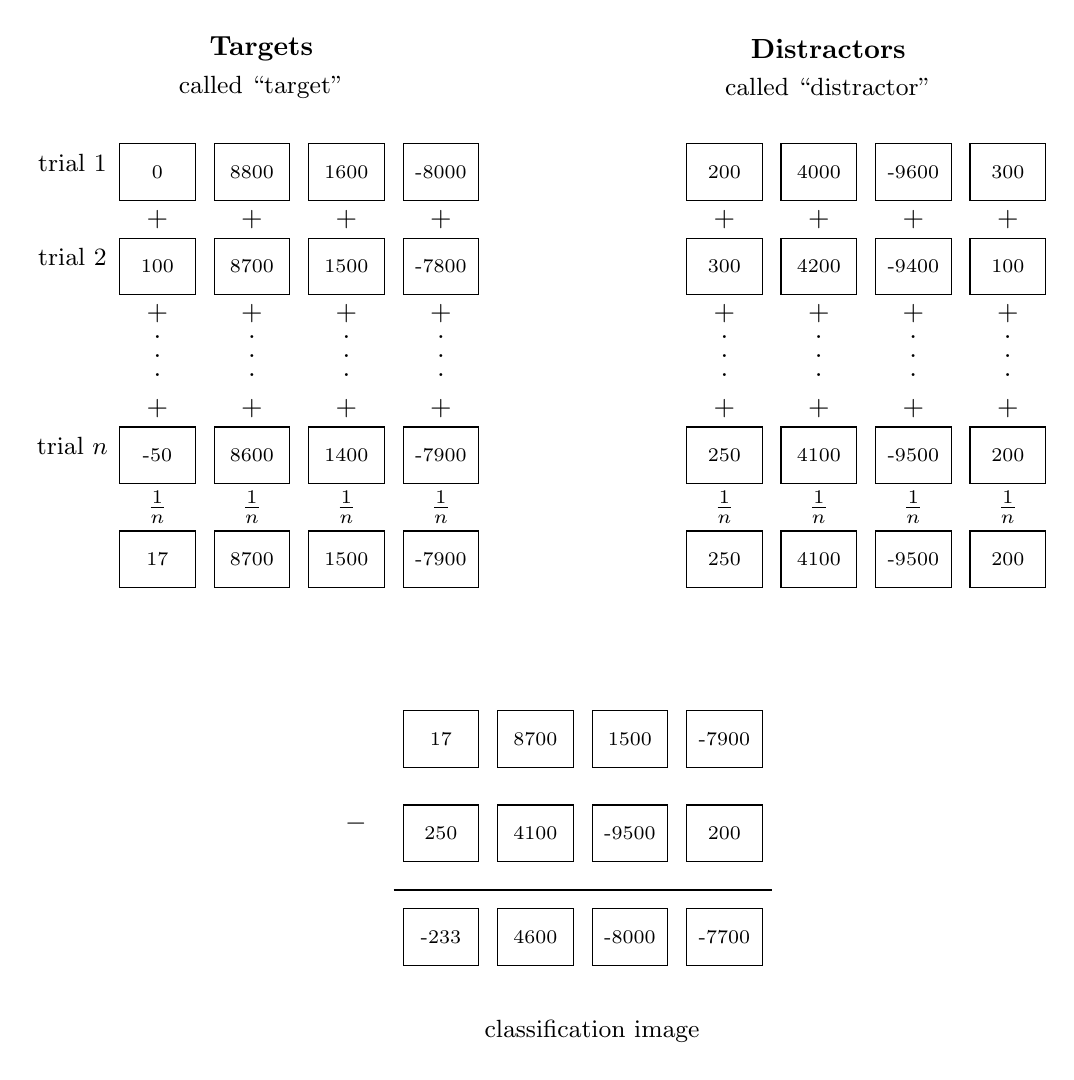
\begin{tikzpicture}[x=1.2cm,y=1.2cm]

% --- HEADERS ---
\node at (0,3.2) {\textbf{Targets}};
\node at (6,3.2) {\textbf{Distractors}};
\node at (0,2.8) {\small called ``target''};
\node at (6,2.8) {\small called ``distractor''};

% --- ROW 1 ---
\node at (-2,2) {\small trial 1};
\foreach \i/\val in {0/0,1/8800,2/1600,3/-8000} {
  \draw (\i-1.5,1.6) rectangle +(0.8,0.6);
  \node at (\i-1.1,1.9) {\scriptsize \val};
}
\foreach \i/\val in {0/200,1/4000,2/-9600,3/300} {
  \draw (\i+4.5,1.6) rectangle +(0.8,0.6);
  \node at (\i+4.9,1.9) {\scriptsize \val};
}

% --- PLUS BETWEEN ROWS ---
\foreach \x in {-1.1,-0.1,0.9,1.9} {
  \node at (\x,1.4) {$+$};
}
\foreach \x in {4.9,5.9,6.9,7.9} {
  \node at (\x,1.4) {$+$};
}

% --- ROW 2 ---
\node at (-2,1) {\small trial 2};
\foreach \i/\val in {0/100,1/8700,2/1500,3/-7800} {
  \draw (\i-1.5,0.6) rectangle +(0.8,0.6);
  \node at (\i-1.1,0.9) {\scriptsize \val};
}
\foreach \i/\val in {0/300,1/4200,2/-9400,3/100} {
  \draw (\i+4.5,0.6) rectangle +(0.8,0.6);
  \node at (\i+4.9,0.9) {\scriptsize \val};
}

% --- PLUS BETWEEN ROWS ---
\foreach \x in {-1.1,-0.1,0.9,1.9} {
  \node at (\x,0.4) {$+$};
}
\foreach \x in {4.9,5.9,6.9,7.9} {
  \node at (\x,0.4) {$+$};
}

% --- ELLIPSIS ---
\foreach \x in {-1.1,-0.1,0.9,1.9} {
  \node at (\x,0.15) {$.$};
}
\foreach \x in {4.9,5.9,6.9,7.9} {
  \node at (\x,0.15) {$.$};
}
\foreach \x in {-1.1,-0.1,0.9,1.9} {
  \node at (\x,-0.05) {$.$};
}
\foreach \x in {4.9,5.9,6.9,7.9} {
  \node at (\x,-0.05) {$.$};
}
\foreach \x in {-1.1,-0.1,0.9,1.9} {
  \node at (\x,-0.25) {$.$};
}
\foreach \x in {4.9,5.9,6.9,7.9} {
  \node at (\x,-0.25) {$.$};
}


% --- PLUS ABOVE LAST ROW ---
\foreach \x in {-1.1,-0.1,0.9,1.9} {
  \node at (\x,-0.6) {$+$};
}
\foreach \x in {4.9,5.9,6.9,7.9} {
  \node at (\x,-0.6) {$+$};
}

% --- LAST ROW ---
\node at (-2,-1) {\small trial $n$};
\foreach \i/\val in {0/-50,1/8600,2/1400,3/-7900} {
  \draw (\i-1.5,-1.4) rectangle +(0.8,0.6);
  \node at (\i-1.1,-1.1) {\scriptsize \val};
}
\foreach \i/\val in {0/250,1/4100,2/-9500,3/200} {
  \draw (\i+4.5,-1.4) rectangle +(0.8,0.6);
  \node at (\i+4.9,-1.1) {\scriptsize \val};
}


% --- 1/n LABEL ---
\foreach \x in {-1.1,-0.1,0.9,1.9,4.9,5.9,6.9,7.9} {
  \node at (\x,-1.65) {$\tfrac{1}{n}$};
}

% --- AVERAGED VECTORS ---
\foreach \i/\val in {0/17,1/8700,2/1500,3/-7900} {
  \draw (\i-1.5,-2.5) rectangle +(0.8,0.6);
  \node at (\i-1.1,-2.2) {\scriptsize \val};
}
\foreach \i/\val in {0/250,1/4100,2/-9500,3/200} {
  \draw (\i+4.5,-2.5) rectangle +(0.8,0.6);
  \node at (\i+4.9,-2.2) {\scriptsize \val};
}


% --- RESTATE NORMALIZED VECTORS FOR SUBTRACTION ---
\foreach \i/\val in {0/17,1/8700,2/1500,3/-7900}  {
  \draw (\i+1.5,-4.4) rectangle +(0.8,0.6);
  \node at (\i+1.9,-4.1) {\scriptsize \val};
}

\node at (1.0,-5.0) {$-$};

\foreach \i/\val in {0/250,1/4100,2/-9500,3/200} {
  \draw (\i+1.5,-5.4) rectangle +(0.8,0.6);
  \node at (\i+1.9,-5.1) {\scriptsize \val};
}

\draw (1.4,-5.7) -- (5.4,-5.7);

\foreach \i/\val in {0/-233,1/4600,2/-8000,3/-7700} {
  \draw (\i+1.5,-6.5) rectangle +(0.8,0.6);
  \node at (\i+1.9,-6.2) {\scriptsize \val};
}

\node at (3.5,-7.2) {\small classification image};
\end{tikzpicture}
\end{center}


So the final row is the classification sound for na given subject. But how do we use this to compare performance against chance?
We start by taking the true classification sound. Generating the true classification sound follows the same exact process as generating the subject's classification sound, except instead of averaging the stimuli that the subject called "target" and "distractor", we average the actual target stimuli and distractor stimuli. This gives us a true target waveform that we can compare against the subject's classification sound.
We compare these two sounds (\textbf{vectors}) using \textbf{cosine similarity}. Cosine similarity between two vectors is the cosine of the angle between them in high-dimensional space. It ranges from $+1$ (identical direction) to $0$ (orthogonal) to $-1$ (opposite direction). We use it to compare a subject's classification image to the true target waveform.

The intuition: a subject's \emph{classification image} is built by
averaging the audio waveforms of all the trials they called ``target''
and subtracting the average of trials they called ``distractor''. If
they were guessing, this difference is just averaged noise and points
in a random direction and you would expect a cosine similarity close to 0. If they were actually picking up on the target,
this then you would see more alignment and you would expect a cosine similarity closer to 1.
If the subject can pick up on the difference between targets and distractors, but they have mislabelled them (they think targets are distractors and vice versa), then you would expect a cosine similarity closer to -1.

Why cosine and not raw dot product: cosine ignores how loud or
contrasty the subject's classification sound happens to be (its
length) and only asks whether it points in the right direction. Two
subjects with very different overall response biases can both have
$\cos = +0.5$ if their classification images both \emph{shape-match}
the target.

Below is a diagram to help you visualize.

\begin{center}
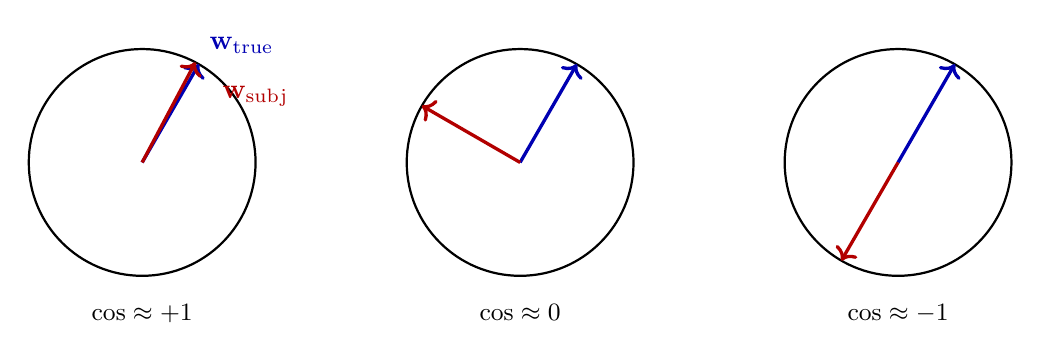
\begin{tikzpicture}[scale=1.2]
  \draw[thick] (0,0) circle (1.2);
  \draw[->, very thick, blue!70!black] (0,0) -- (60:1.2)
        node[above right]{$\mathbf{w}_{\text{true}}$};
  \draw[->, very thick, red!70!black] (0,0) -- (62:1.2);
  \node[red!70!black] at (1.2,0.7) {$\mathbf{w}_{\text{subj}}$};
  \node[below] at (0,-1.4) {\small $\cos \approx +1$};

  \begin{scope}[xshift=4cm]
    \draw[thick] (0,0) circle (1.2);
    \draw[->, very thick, blue!70!black] (0,0) -- (60:1.2);
    \draw[->, very thick, red!70!black] (0,0) -- (150:1.2);
    \node[below] at (0,-1.4) {\small $\cos \approx 0$};
  \end{scope}

  \begin{scope}[xshift=8cm]
    \draw[thick] (0,0) circle (1.2);
    \draw[->, very thick, blue!70!black] (0,0) -- (60:1.2);
    \draw[->, very thick, red!70!black] (0,0) -- (240:1.2);
    \node[below] at (0,-1.4) {\small $\cos \approx -1$};
  \end{scope}
\end{tikzpicture}
\end{center}

\subsection{$d'$ (signal-detection sensitivity)}

Accuracy alone can lie to you. Imagine two subjects who both score $0.55$:
\begin{itemize}
  \item \textbf{Subject A} is balanced. When the trial really was a target they call it ``target'' about $55\%$ of the time, and when it really was a distractor they call it ``distractor'' about $55\%$ of the time. They are slightly but genuinely picking up on something.
  \item \textbf{Subject B} just likes the ``target'' button. They press it on almost every trial. They get nearly every real target right (great hit rate!) but they also call most distractors targets too (terrible false-alarm rate). The two errors partly cancel and they end up at $0.55$ accuracy as well.
\end{itemize}
Same accuracy, very different subjects. We want a number that rewards Subject A and not Subject B; a number that asks ``can you actually tell the two classes apart?'' separately from ``which button do you tend to press?''. That number is $d'$ (pronounced ``d-prime''), the standard sensitivity measure from signal-detection theory.

The two ingredients are:
\begin{itemize}
  \item the \textbf{hit rate} $H = P(\text{say ``target''} \mid \text{trial really was a target})$, and
  \item the \textbf{false-alarm rate} $F = P(\text{say ``target''} \mid \text{trial really was a distractor})$.
\end{itemize}
A subject who can truly discriminate has $H$ noticeably larger than $F$. A subject who is just guessing or just pressing one button has $H \approx F$, no matter what that shared value is.

$d'$ formalises ``how much bigger is $H$ than $F$'' on a $z$-score scale:
\[
d' = z(H) - z(F),
\]
where $z(\cdot)$ is the inverse of the standard normal CDF. Putting things on the $z$-scale just means we're measuring the gap between $H$ and $F$ in standard-deviation units of an underlying ``evidence'' axis, which is the natural scale if you imagine targets and distractors producing two overlapping bell curves of internal evidence and the subject placing a single decision threshold somewhere on that axis.

The intuition picture: imagine two bell curves on an internal ``how target-like did this sound?'' axis: one for distractor trials, one for target trials. $d'$ is just the distance between the centers of those two bells, in units of their width. $d' = 0$ means the bells sit on top of each other (no discrimination, regardless of where the subject's button-press cutoff sits). $d' = 1$ means the target bell has slid one full standard deviation to the right of the distractor bell. Bigger $d'$ = the two classes feel more distinct internally.

\begin{center}
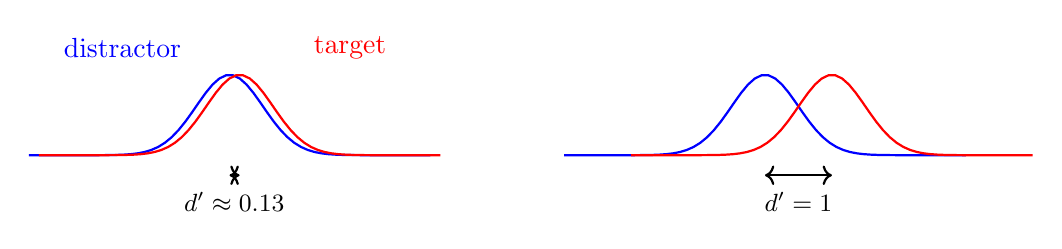
\begin{tikzpicture}[scale=0.85]
  \def\bell#1#2{\draw[#2, thick] plot[domain=-3:3, samples=60] (\x+#1, {1.2*exp(-(\x)^2/0.5)});}
  \bell{0}{blue}
  \bell{0.15}{red}
  \node[blue] at (-1.6, 1.6) {distractor};
  \node[red]  at ( 1.8, 1.6) {target};
  \draw[<->, thick] (0, -0.3) -- (0.15, -0.3);
  \node at (0.07, -0.7) {\small $d' \approx 0.13$};

  \begin{scope}[xshift=8cm]
    \bell{0}{blue}
    \bell{1}{red}
    \draw[<->, thick] (0, -0.3) -- (1, -0.3);
    \node at (0.5, -0.7) {\small $d' = 1$};
  \end{scope}
\end{tikzpicture}
\end{center}

Null value is $d' = 0$ (no ability to discriminate). As a sanity check that ties this back to the accuracy section: a subject scoring $0.526$ with no response bias corresponds to $d' \approx 0.13$, which is exactly what we see for the Oberlin full-sentence row in Section~E.\@ So $d'$ and accuracy will track each other when subjects are unbiased; $d'$ only really earns its keep when a subject is leaning hard on one button, in which case it punishes the bias and accuracy doesn't.

\subsection{$\beta_{\text{truetarget}}$ (regression slope on the true target)}

The classification image from the previous subsection is one way to ask ``did this subject's responses line up with the true target?'', but it does so by collapsing all of the subject's ``target'' trials into one big average. $\beta_{\text{truetarget}}$ asks the same question \emph{trial by trial} instead.

Here is the intuition. For every single trial, take the white-noise stimulus the subject heard on that trial and compute its dot product with the true target waveform. That single number says ``how much did this particular noise clip resemble the true target?'' A big positive number means it looked a lot like the target, near zero means it didn't, negative means it looked like the opposite. Now line up, for that same subject, all 149 of those similarity scores against the binary response they actually gave (1 if they said ``target'', 0 if they said ``distractor''), and fit a logistic regression:
\[
P(\text{response = ``target''}) = \text{logistic}\bigl(\alpha + \beta_{\text{truetarget}} \cdot \text{(similarity to true target on this trial)}\bigr).
\]
The slope $\beta_{\text{truetarget}}$ is what we care about. It directly answers: \emph{the more a trial's audio resembled the true target, the more likely was this subject to press ``target''?}

Reading the slope:
\begin{itemize}
  \item $\beta_{\text{truetarget}} > 0$: yes, target-like trials drove ``target'' responses. The subject is tracking the true signal.
  \item $\beta_{\text{truetarget}} \approx 0$: no relationship. Whether a clip resembled the target or not had no bearing on what the subject pressed.
  \item $\beta_{\text{truetarget}} < 0$: the relationship runs backwards (target-like clips made the subject \emph{less} likely to say ``target''), which would be weird and would suggest the subject's internal template is anti-aligned.
\end{itemize}
Null value is $0$. The units are log-odds per unit of target-similarity: a slope of $0.232$ (Oberlin, Section~E) means that increasing a trial's similarity to the true target by one similarity-unit multiplies the odds the subject calls it ``target'' by $e^{0.232} \approx 1.26$.

Why bother with this on top of the classification image and $d'$? Because it is the most direct test of the hypothesis. The classification image asks ``does the average of your `target' calls look like the target?'' and $d'$ asks ``can you tell the two labelled classes apart?''. $\beta_{\text{truetarget}}$ asks the cleanest version of the question: trial by trial, when the noise actually happened to look like the target, did you notice? If all three metrics point the same way, that is convergent evidence that the subject is genuinely picking up on the target structure rather than on some incidental feature of the labels.

%==============================================================================
\section{Results}
%==============================================================================

\subsection{Section A: Accuracy vs chance}

\begin{numbersbox}[Section A (\texttt{A\_accuracy\_vs\_chance.csv})]
\centering\small
\begin{tabular}{llrrlrr}
\toprule
block & group & $n$ & mean & 95\% CI & Wilcoxon $p$ & $d$ \\
\midrule
full\_sentence     & UChicago & 10 & 0.504 & $[0.479, 0.530]$ & 0.869  & $+0.09$ \\
full\_sentence     & Oberlin  & 16 & 0.526 & $[0.513, 0.538]$ & 0.0037 & $+0.99$ \\
full\_sentence     & Unified  & 26 & 0.518 & $[0.504, 0.530]$ & 0.019  & $+0.50$ \\
imagined\_sentence & UChicago & 10 & 0.490 & $[0.464, 0.515]$ & 0.611  & $-0.23$ \\
imagined\_sentence & Oberlin  & 16 & 0.510 & $[0.495, 0.526]$ & 0.277  & $+0.31$ \\
imagined\_sentence & Unified  & 26 & 0.502 & $[0.488, 0.517]$ & 0.517  & $+0.06$ \\
\bottomrule
\end{tabular}
\end{numbersbox}

\begin{figure}[h]
\centering
\includegraphics[width=\linewidth]{A_accuracy_vs_chance.png}
\caption{Per-subject accuracy by (block, group). Red dashed = chance
($0.50$); black solid = group mean. Title shows the bootstrap CI on the
mean and the Wilcoxon $p$ vs.\ chance.}
\end{figure}

Bonferroni-corrected threshold across the six tests is
$\alpha = 0.05/6 \approx 0.0083$. Oberlin full-sentence
($p = 0.0037$) clears it; the Unified full-sentence cell
($p = 0.019$) does not.

\subsection{Section B: Full vs Imagined (paired)}

\begin{numbersbox}[Section B (\texttt{B\_full\_vs\_imagined.csv})]
\centering\small
\begin{tabular}{lrrrrrrr}
\toprule
group & $n$ & mean(F) & mean(I) & mean diff & paired Wilcoxon $p$ & perm $p$ & $d$ \\
\midrule
UChicago & 10 & 0.504 & 0.490 & $+0.0141$ & 0.543 & 0.508 & $+0.22$ \\
Oberlin  & 16 & 0.526 & 0.510 & $+0.0159$ & 0.209 & 0.198 & $+0.35$ \\
Unified  & 26 & 0.518 & 0.502 & $+0.0152$ & 0.157 & 0.158 & $+0.29$ \\
\bottomrule
\end{tabular}
\end{numbersbox}

\begin{figure}[h]
\centering
\includegraphics[width=\linewidth]{B_full_vs_imagined.png}
\caption{Per-subject lines connecting Full to Imagined accuracy in each
group; coloured heavy line is the group mean.}
\end{figure}

The mean difference is $+0.0152$ pooled and positive in both sites.
No paired test reaches $p < 0.05$.

\subsection{Section C: Site comparison}

\begin{numbersbox}[Section C (\texttt{C\_site\_comparison.csv})]
\centering\small
\begin{tabular}{lrrrrrrrr}
\toprule
block & $n_O$ & $n_U$ & mean$_O$ & mean$_U$ & diff & MWU $p$ & Welch $p$ & $d$ \\
\midrule
full\_sentence     & 16 & 10 & 0.526 & 0.504 & $+0.0220$ & 0.145 & 0.173 & $+0.65$ \\
imagined\_sentence & 16 & 10 & 0.510 & 0.490 & $+0.0201$ & 0.475 & 0.231 & $+0.54$ \\
\bottomrule
\end{tabular}
\end{numbersbox}

\begin{figure}[h]
\centering
\includegraphics[width=0.85\linewidth]{C_site_comparison.png}
\caption{Per-block boxplots, Oberlin vs.\ UChicago, with overlaid
jittered subject points.}
\end{figure}

Oberlin is numerically higher than UChicago in both blocks by
$\approx 0.02$. Neither between-site comparison reaches $p < 0.05$.

\subsection{Section D: Block order}

\begin{numbersbox}[Section D selected rows (\texttt{D\_block\_order.csv})]
\centering\small
\begin{tabular}{llrrrrrr}
\toprule
block & group & $n_{B1}$ & $n_{B2}$ & mean(B1) & mean(B2) & MWU $p$ & $d$ \\
\midrule
full\_sentence     & Oberlin  &  5 & 11 & 0.519 & 0.529 & 0.493 & $+0.35$ \\
imagined\_sentence & Oberlin  & 11 &  5 & 0.500 & 0.532 & 0.078 & $+1.03$ \\
\bottomrule
\end{tabular}
\end{numbersbox}

In the Oberlin imagined block, subjects who completed it second
($n_{B2}=5$) averaged $0.532$, vs $0.500$ for those who completed it
first ($n_{B1}=11$); MWU $p = 0.078$, $d = +1.03$. All other
block-order cells have $p > 0.4$.

\subsection{Section E: Convergent metrics, full-sentence block}

\begin{numbersbox}[Section E (\texttt{E\_convergent\_full\_sentence.csv})]
\centering\small
\begin{tabular}{llrrrr}
\toprule
group & metric & mean & 95\% CI & Wilcoxon $p$ & $d$ \\
\midrule
Oberlin  & d$'$              & $+0.137$ & $[+0.069, +0.200]$ & 0.0013 & $+0.99$ \\
Oberlin  & accuracy          & $+0.526$ & $[+0.513, +0.538]$ & 0.0037 & $+0.99$ \\
Oberlin  & cos(CI, true)     & $+0.056$ & $[+0.029, +0.083]$ & 0.0013 & $+1.00$ \\
Oberlin  & beta\_truetarget  & $+0.232$ & $[+0.118, +0.340]$ & 0.0027 & $+0.99$ \\
\midrule
UChicago & d$'$              & $+0.021$ & $[-0.106, +0.153]$ & 0.846  & $+0.09$ \\
UChicago & cos(CI, true)     & $-0.002$ & $[-0.059, +0.056]$ & 1.000  & $-0.02$ \\
UChicago & beta\_truetarget  & $+0.042$ & $[-0.159, +0.248]$ & 0.846  & $+0.12$ \\
\midrule
Unified  & d$'$              & $+0.093$ & $[+0.023, +0.159]$ & 0.013  & $+0.51$ \\
Unified  & cos(CI, true)     & $+0.034$ & $[+0.004, +0.063]$ & 0.025  & $+0.43$ \\
Unified  & beta\_truetarget  & $+0.159$ & $[+0.047, +0.267]$ & 0.016  & $+0.55$ \\
\bottomrule
\end{tabular}
\end{numbersbox}

\begin{figure}[h]
\centering
\includegraphics[width=\linewidth]{E_convergent_full_sentence.png}
\caption{Each row is a metric, each column a group. Red dashed = null
value (0 or 0.5); black solid = observed mean.}
\end{figure}

At Oberlin all four metrics yield $p \le 0.0037$ and $d \approx 1.0$.
At UChicago all four are non-significant with $|d| \le 0.12$. Pooled,
all four yield $p \in [0.013, 0.025]$ and $d \in [0.43, 0.55]$.

\subsection{Section F: Questionnaire correlations}

48 Spearman correlations (8 questionnaires $\times$ 2 blocks $\times$
3 groups). Bonferroni threshold $p < 0.001$. None survive correction.
Tables: \texttt{F\_questionnaire\_spearman.csv}; figures:
\texttt{F\_quest\_vs\_accuracy\_full\_sentence.png},
\texttt{F\_quest\_vs\_accuracy\_imagined\_sentence.png}.

%==============================================================================
\section{Further analyses available with the existing data}
%==============================================================================

\subsection{Trial-by-trial mixed-effects modelling}

The current per-subject summaries collapse $\sim$150 trials per block
into a single mean. A mixed-effects logistic regression on raw trials,
with subject as a random effect, would use the within-subject trial
variance directly.

\subsection{Bayesian re-analysis of trending comparisons}

For comparisons with $0.05 < p < 0.20$ (Section~B Full--Imagined paired,
Section~C site differences), Bayes factors quantify the evidence ratio
between $H_1$ and $H_0$ rather than only rejecting $H_0$.

\subsection{Within-subject correlations between convergent metrics}

The four Section~E metrics are tested independently. Computing the
per-subject correlation matrix between $d'$, accuracy, $\cos(\mathrm{CI},
\text{true})$, and $\beta_{\text{truetarget}}$ tests whether they are
driven by a single latent perceptual ability.

\subsection{Spectral classification image}

A 32-band spectral analogue of the time-domain classification image: for
each subject, fit per-band weights and compute the cosine with the true
target's per-band spectrum.

\begin{center}
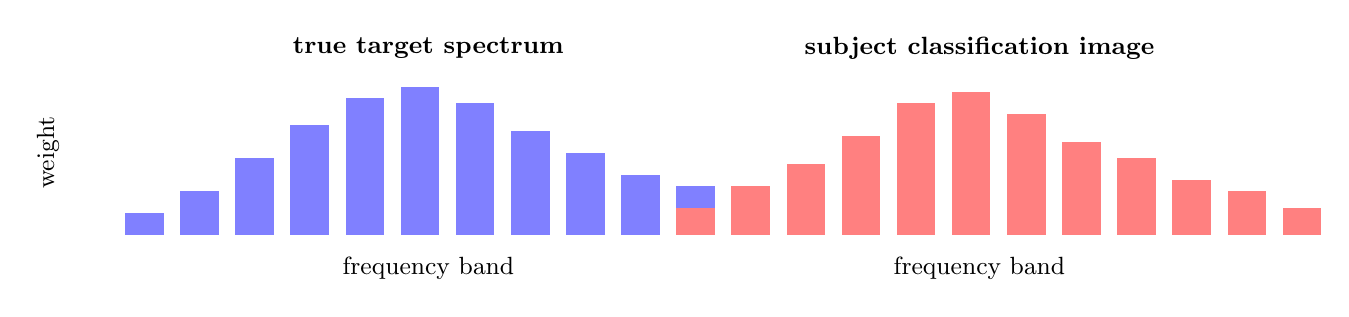
\begin{tikzpicture}[scale=0.7]
  \foreach \x/\h in {1/0.4, 2/0.8, 3/1.4, 4/2.0, 5/2.5, 6/2.7,
                     7/2.4, 8/1.9, 9/1.5, 10/1.1, 11/0.9, 12/0.6}
    \fill[blue!50] (\x,0) rectangle (\x+0.7, \h);
  \node at (6.5,-0.6) {\small frequency band};
  \node[rotate=90] at (-0.4,1.5) {\small weight};
  \node at (6.5,3.4) {\small \textbf{true target spectrum}};

  \begin{scope}[xshift=10cm]
    \foreach \x/\h in {1/0.5, 2/0.9, 3/1.3, 4/1.8, 5/2.4, 6/2.6,
                       7/2.2, 8/1.7, 9/1.4, 10/1.0, 11/0.8, 12/0.5}
      \fill[red!50] (\x,0) rectangle (\x+0.7, \h);
    \node at (6.5,-0.6) {\small frequency band};
    \node at (6.5,3.4) {\small \textbf{subject classification image}};
  \end{scope}
\end{tikzpicture}
\end{center}

\subsection{Block-order follow-up in the Oberlin imagined block}

Trial-resolved analysis of the $n_{B2}=5$ vs $n_{B1}=11$ split: e.g.\
within-block accuracy time course, and whether the $+0.032$ mean
difference is concentrated in early or late trials of the block.

\subsection{Stimulus-level analyses}

Per-stimulus accuracy across the audio set, to test whether particular
target/distractor pairs drive the Oberlin full-sentence effect.
Building blocks for this exist in \texttt{stimuli-analyses/}
(classification-image, spectral logistic, etc.).

\end{document}
